\documentclass[11pt]{article}

\usepackage[margin=1in]{geometry}
\usepackage{amsmath,amssymb}
\usepackage{booktabs}
\usepackage{graphicx}
\usepackage{xcolor}
\usepackage{tikz}
\usetikzlibrary{patterns,arrows.meta,positioning,calc}
\usepackage{pgfplots}
\pgfplotsset{compat=1.16}
\usepackage{hyperref}
\hypersetup{colorlinks=true,linkcolor=blue,citecolor=blue,urlcolor=blue}
\usepackage{caption}
\usepackage{enumitem}

\newcommand{\Rsq}{R^{2}}
\newcommand{\redbox}[1]{\textcolor{red!70!black}{\textbf{#1}}}
\newcommand{\greenbox}[1]{\textcolor{green!45!black}{\textbf{#1}}}

\title{\textbf{The Non-Invasive Depth Wall:\\
An In-Silico Negative Result on Reaching Invasive-Grade\\
Brain Access From Outside the Skull, With a Cortical-Surface\\
Capability Window and a Read/Write Depth Asymmetry}}

\author{anima AURA domain \\ \texttt{github.com/dancinlab/anima}}
\date{2026-05-30}

\begin{document}
\maketitle

\begin{abstract}
We ask, as a pre-registered falsification test, whether a strictly non-invasive
interface (behind-the-ear and high-density scalp electrode arrays, plus
heterogeneous read/write modalities) can reach the access grade of invasive
hardware (electrocorticography, ECoG; depth/stereo-EEG) --- in particular whether
it can read or write \emph{deep} (sub-cortical / nuclear) brain structures. The
falsifier was pre-registered: the hypothesis survives if the active-source recovery
rate fails to collapse with depth, or if non-invasive deep \emph{reading} is
demonstrably possible. We test it in silico with two forward head models --- a
Gaussian-blur projection and a physically grounded three-shell concentric-sphere
lead field (Ary--Klein--Fender 1981 geometry) --- and a family of inverse solvers
(ridge / minimum-norm, ISTA/IRLS, and an oracle upper bound), scoring active-source
recovery by $\Rsq$. The result is a \redbox{closed-negative}: under the physically
grounded three-shell model the cortical-surface-to-deep-nucleus recovery ratio is
$0.239 \rightarrow 0.016$ ($\times 15.4$ collapse) across the full source-eccentricity
sweep --- \emph{steeper}, not gentler, than the Gaussian best-envelope's
$0.820 \rightarrow 0.098$ ($\times 8.4$). The apparent ``electrode saturation'' that
the Gaussian model shows is revealed to be a \emph{modelling artifact} that the
three-shell model does not reproduce (recovery keeps rising, $0.19 \rightarrow 0.40$,
out to 1024 contacts). The depth wall is therefore a real physical boundary, not a
solver or sampling deficiency: deep robustly under-recovers cortex in both models.
This independently converges with the AURA B7 intracortical-ceiling finding. We then
report two positive complements. First, on the \emph{cortical surface}, stacking
heterogeneous modalities and priors closes much of the gap to invasive grade
(EEG $0.329 \rightarrow$ full-stack$+$time $0.820$ at the cortical layer; tFUS adds
the best deep-residual lever; channel density is a real, non-saturating lever under
faithful physics), defining a \greenbox{near-invasive cortical-surface capability
window}. Second, the only non-invasive route that \emph{touches} the deep brain is a
\emph{write} channel (transcranial focused ultrasound, tFUS, best deep $\Rsq\approx
0.15$--$0.20$), not a read channel (deep read is the empty quadrant) --- a read/write
depth asymmetry. We state all numerical results as $\Rsq$ on a spherical,
Gaussian-source toy head; real-head, real-data, and built-in $\Phi$ confirmation are
explicitly NOT-MEASURED. The qualitative rulings (deep $<$ cortex robustly;
saturation is an artifact; cortical stacking helps; write-only deep route) are robust
to these caveats.
\end{abstract}

\tableofcontents
\bigskip

%==========================================================================
\section{Introduction}
\label{sec:intro}

The AURA program asks a single load-bearing engineering question: can a brain
interface that never breaks the skin --- electrodes resting behind the ear or in a
high-density scalp cap, supplemented by trans-skull read/write physics --- be pushed
to the access grade of \emph{invasive} hardware? Invasive grade here means two
things at once: (i) the spatial fidelity of ECoG grids sitting directly on cortex,
and (ii) the reach of depth / stereo-EEG and deep-brain-stimulation (DBS) leads into
sub-cortical nuclei. If the answer were yes, the entire ``whole-brain control via
relocation'' premise --- keep an N1-class chip but move it, or skip the chip and use
external fields --- would be on the table. If the answer is no, the negative result
is itself the finding: it deterministically rules out an axis and forces the program
onto the surviving branches.

This paper is the C-axis (``non-invasive $\rightarrow$ invasive-grade'') counterpart
to the previously shipped A-axis paper on scalp electrode-position $\Phi$-proxy
mapping. It is \emph{not} a duplicate: the A-axis paper measured how electrode
\emph{position} on the scalp shapes a consciousness proxy; this paper measures the
\emph{depth} dimension --- how far in, and in which direction (read vs.\ write), a
non-invasive interface can reach, and where the wall is.

\paragraph{Three claims.} We make one negative claim and two positive complements:
\begin{enumerate}[leftmargin=2em]
  \item \redbox{Closed-negative:} non-invasive whole-brain (deep) control is
        physically walled. Active-source recovery collapses with depth, and the
        collapse is steeper, not gentler, when the head model is made physically
        faithful. The wall is real, not an artifact of a weak solver or sparse
        sampling.
  \item \greenbox{Cortical-surface capability window:} on the cortical surface,
        heterogeneous modality fusion plus priors brings non-invasive recovery
        close to invasive grade --- a genuine application regime.
  \item \textbf{Read/write asymmetry:} the only non-invasive channel that reaches
        deep structures is a \emph{write} channel (tFUS neuromodulation), not a read
        channel. Deep reading is the hard-walled direction.
\end{enumerate}

\paragraph{Honesty frame.} Every number below is an $\Rsq$ active-source-recovery
score computed on a \emph{spherical, Gaussian-source toy head} with synthetic
sources --- a deliberately simple in-silico testbed. Real skull anisotropy, real
gyral folding, real recorded data, and a hardware-/builtin-verified $\Phi$ are
\textbf{NOT-MEASURED} in this work. We argue (Section~\ref{sec:threats}) that the
qualitative rulings survive these simplifications precisely because making the model
\emph{more} realistic (Gaussian $\rightarrow$ three-shell) made the wall
\emph{stronger}, not weaker.

%==========================================================================
\section{Pre-Registered Hypothesis and Falsifier}
\label{sec:hypothesis}

\paragraph{Hypothesis $H$ (the optimistic claim under test).}
A strictly non-invasive interface --- behind-the-ear plus high-density scalp arrays,
optionally augmented by trans-skull read/write modalities --- can reach
\emph{invasive-grade} access, including the ability to \emph{read} deep
(sub-cortical / nuclear) structures, such that active-source recovery does
\emph{not} collapse as the source depth increases.

\paragraph{Pre-registered falsifier $F$.} $H$ \emph{survives} (is corroborated) if
\emph{either}:
\begin{itemize}[leftmargin=2em]
  \item[\textbf{F1}] the active-source recovery rate $\Rsq(d)$ does \emph{not}
        collapse as depth $d$ increases --- operationally, the
        cortical-to-deep ratio stays within a small factor ($\lesssim 2\times$)
        under a physically faithful head model; \emph{or}
  \item[\textbf{F2}] non-invasive \emph{deep reading} is demonstrably possible ---
        some non-invasive read modality recovers a deep source at cortical-grade
        $\Rsq$.
\end{itemize}
$H$ is \redbox{falsified} if the depth collapse is large \emph{and} steepens (or at
least does not soften) when the head model is made more physically realistic,
\emph{and} no non-invasive read modality reaches deep structures.

This is a genuine pre-registration: the falsifier is stated as a numerical threshold
on a quantity ($\Rsq$ ratio vs.\ depth) that the experiment then measures, and the
direction that would have rescued $H$ (the ratio \emph{shrinking} under a better
model) is exactly the direction we did not observe. Indeed, an intermediate AURA
round (AURA-HEADMODEL) explicitly conjectured that the Gaussian toy
\emph{over-states} the depth wall --- the conjecture that would have triggered F1 ---
and that conjecture was itself falsified by sign reversal (Section~\ref{sec:depthwall}).

%==========================================================================
\section{Method}
\label{sec:method}

\subsection{Forward models (head $\rightarrow$ sensor)}
We instantiate two forward operators mapping a source configuration to scalp sensor
readings.

\paragraph{(M1) Gaussian-blur projection.} A phenomenological forward operator in
which each source contributes to each sensor through an isotropic Gaussian kernel,
$\exp(-d^2/2\sigma^2)$, of the source--sensor distance $d$. This is the ``naive''
model: it captures distance-dependent attenuation but \emph{not} the conductivity
structure of the head.

\paragraph{(M2) Three-shell concentric-sphere lead field.} A physically grounded
forward model using the Ary--Klein--Fender (1981) three-shell concentric-sphere
geometry: brain ($r_1=8.0$\,cm), skull ($r_2=8.5$\,cm,
$\sigma_{\text{skull}}=\sigma_{\text{brain}}/40$), and scalp ($r_3=9.2$\,cm) shells.
A radial dipole at brain-internal radius $b$ produces a scalp potential as a Legendre
series $V(\theta)=\sum_n g_n P_n(\cos\theta)$, where the coefficients $g_n$ are set
by the conductivity ratio and the radius ratios. The low skull conductivity plus
source eccentricity attenuate high spatial-frequency terms (high $n$), so a
\emph{physical} spatial low-pass filter (LPF) arises \emph{without} any Gaussian
assumption. The radial-dipole scalp trace scales as $g_n \propto b^{2n}$, so as the
source moves deep ($b\to 0$) the high-$n$ content vanishes. This is the standard
analytic head model used as the validation baseline before realistic
boundary-element / finite-element models~\cite{ary1981,nunez2006,darvas2004}.

\subsection{Inverse solvers (sensor $\rightarrow$ source estimate)}
Given the simulated sensor vector we recover a source estimate with a family of
inverse operators, so that the depth wall cannot be blamed on a single weak solver:
\begin{itemize}[leftmargin=2em]
  \item \textbf{Ridge / minimum-norm} --- the regularised least-squares
        $\hat{x} = L^{\!\top}(LL^{\!\top}+\lambda I)^{-1} y$ baseline;
  \item \textbf{ISTA / IRLS} --- a sparsity-leaning solver that should favour focal
        deep sources if they were recoverable (in our sweeps, $L1$/ISTA
        \emph{under}performed ridge at all depths --- a dead end, not a rescue);
  \item \textbf{Oracle} --- an upper bound told the true support, isolating the
        information-theoretic ceiling of the forward operator from solver
        limitations.
\end{itemize}

\subsection{Scoring}
For an active source at depth (eccentricity) $d$, we score recovery by the
coefficient of determination $\Rsq(d)$ between the true and recovered source activity
over the active support. $\Rsq = 1$ is perfect recovery; $\Rsq = 0$ is chance. We
average over 8 random seeds (synthetic source placements and noise draws, SNR
20\,dB) per operating point. All runs are CPU numpy on the AURA pool host (ubu-1);
no GPU, \$0.

\subsection{Modalities}
Beyond electric scalp potential (EEG), we model heterogeneous read/write channels:
magnetic (room-temperature-superconductor MEG, ``RTSC-MEG''), optically-pumped
magnetometry (OPM-MEG), and --- critically for the asymmetry result --- transcranial
focused ultrasound (tFUS) as a \emph{write} (neuromodulation) channel. Heterogeneous
modalities are fused at the inverse stage.

\subsection{Provenance}
Every numerical result quoted in Section~\ref{sec:measurement} is taken verbatim
from an AURA origin/main verdict ledger:
\texttt{AURA/C15-depth-wall-terminal.md},
\texttt{AURA/AURA-DEPTH/DEPTH-3SHELL-CORRECTION.md},
\texttt{AURA/AURA-HEADMODEL/SPHERE-VALIDATION.md},
\texttt{AURA/C6-multimodal-breakthrough.md},
\texttt{AURA/C7-prior-stack-levers.md},
\texttt{AURA/C16-cortical-capability-map.md},
\texttt{AURA/B7-intracortical-ceiling.md}, and the cross-index
\texttt{AURA/AURA-AXES-INDEX.md}. No number in this paper is generated by the paper
itself.

%==========================================================================
\section{Measurement}
\label{sec:measurement}

\subsection{The depth wall (M1 vs.\ M2)}
\label{sec:depthwall}

Table~\ref{tab:depthwall} reports the headline measurement: active-source recovery
across the full source-eccentricity sweep (cortical surface to deep nucleus) under
each forward model, taken from the three-shell correction ledger.

\begin{table}[h]
\centering
\caption{Active-source recovery $\Rsq$ vs.\ source eccentricity (ecc; $0.95=$
cortical surface, $0.10=$ deep nucleus), three-shell vs.\ in-harness Gaussian, plus
the Ary $g_n$ spatial-spectrum cutoff. Source:
\texttt{AURA/AURA-DEPTH/DEPTH-3SHELL-CORRECTION.md},
\texttt{AURA/C15-depth-wall-terminal.md}.}
\label{tab:depthwall}
\begin{tabular}{lccc}
\toprule
ecc (depth) & M2 three-shell $\Rsq$ & M1 Gaussian (in-harness) $\Rsq$ & cutoff $n$ \\
\midrule
$0.95$ (cortical surface) & $0.239 \pm 0.046$ & $0.119 \pm 0.052$ & $19$ \\
$0.70$ (cortex)           & $0.107 \pm 0.053$ & $0.094 \pm 0.049$ & $8$  \\
$0.50$ (subcortical)      & $0.068 \pm 0.043$ & $0.064 \pm 0.041$ & $6$  \\
$0.30$ (deep)             & $0.051 \pm 0.035$ & $0.052 \pm 0.039$ & $4$  \\
$0.10$ (deep nucleus)     & $\mathbf{0.016 \pm 0.009}$ & $0.038 \pm 0.031$ & $3$ \\
\midrule
cortex$\to$deep ratio & $\mathbf{\times 15.4}$ & $\times 3.2$ & --- \\
\bottomrule
\end{tabular}
\end{table}

\begin{table}[h]
\centering
\caption{Depth-collapse factor by model. The physically faithful three-shell model
collapses \emph{harder} than either Gaussian variant. Source:
\texttt{DEPTH-3SHELL-CORRECTION.md}.}
\label{tab:ratio}
\begin{tabular}{lc}
\toprule
Model & cortex $\to$ deep collapse \\
\midrule
M2 three-shell (physics)            & $\mathbf{\times 15.4}$ \ ($0.239\to0.016$) \\
M1 Gaussian (same harness)          & $\times 3.2$ \ ($0.119\to0.038$) \\
M1 Gaussian (C15 published best-env)& $\times 8.4$ \ ($0.820\to0.098$) \\
\bottomrule
\end{tabular}
\end{table}

The key comparison is the collapse factor. Making the head model physically faithful
\emph{increases} the depth collapse to $\times 15.4$, exceeding even the
strongest-stack Gaussian best-envelope ($\times 8.4$). The deep nucleus recovers at
$\Rsq = 0.016$ --- essentially chance --- under the realistic model, and the
spatial-spectrum cutoff narrows from $n=19$ (surface) to $n=3$ (deep), the
mechanistic signature of the $b^{2n}$ scalp-trace decay. Figure~\ref{fig:wall} plots
the recovery curve for both models.

The C15 full-stack best-envelope (all working levers: RTSC-MEG, tFUS, OPM-MEG, and
the dynamic-time joint-support lever combined) reaches $0.820$ at the cortical layer
but still falls to $0.098$ at the deep nucleus --- the time lever's gain itself
evaporates with depth ($+0.184$ at cortex to $+0.014$ at the deep nucleus). No lever
breaks the wall.

\subsection{Electrode ``saturation'' is a Gaussian artifact}
\label{sec:saturation}

The Gaussian model exhibits an apparent \emph{saturation}: beyond a certain electrode
count, adding contacts stops improving recovery, which would superficially suggest a
hardware-side ceiling. The sphere-validation ledger
(\texttt{AURA/AURA-HEADMODEL/SPHERE-VALIDATION.md}) shows this saturation
\emph{does not appear} in the three-shell model (Table~\ref{tab:saturation}): the
physical model keeps gaining as contacts grow, with the per-doubling increment
\emph{widening} ($+0.075$, $+0.093$) at high $M$, while the Gaussian increment
collapses ($+0.022$). The saturation is a modelling artifact of the isotropic
Gaussian kernel, not a physical property of non-invasive sensing. This matters for
the falsifier: it removes a spurious ``ceiling'' explanation and isolates the depth
collapse as the genuine boundary.

\begin{table}[h]
\centering
\caption{Electrode-count scaling at fixed depth: recovery $\Rsq$ vs.\ number of
contacts $M$. Three-shell does not saturate; Gaussian does. Source:
\texttt{SPHERE-VALIDATION.md} (Q2).}
\label{tab:saturation}
\begin{tabular}{lcccc}
\toprule
$M$ & 3-shell $\Rsq$ & $\Delta$ & Gaussian $\Rsq$ & $\Delta$ \\
\midrule
$8$    & $0.189$ & ---      & $0.136$ & ---      \\
$16$   & $0.222$ & $+0.033$ & $0.143$ & $+0.007$ \\
$64$   & $0.233$ & $+0.012$ & $0.155$ & $+0.012$ \\
$256$  & $0.308$ & $+0.075$ & $0.196$ & $+0.041$ \\
$1024$ & $\mathbf{0.401}$ & $\mathbf{+0.093}$ & $0.218$ & $+0.022$ \\
\bottomrule
\end{tabular}
\end{table}

\subsection{Cortical-surface heterogeneous-modality fusion}
\label{sec:cortical}

On the \emph{cortical surface} (not deep), stacking modalities and priors recovers
much of the gap to invasive grade. Table~\ref{tab:cortical} collects the levers from
the depth-wall ledger.

\begin{table}[h]
\centering
\caption{Cortical-layer ($d\!=\!1.5$) and deep-nucleus ($d\!=\!8.0$) recovery by
modality, and the full-stack best-envelope across depth. Sources:
\texttt{AURA/C15-depth-wall-terminal.md} (modal columns, time lever, best-envelope),
\texttt{AURA/C16-cortical-capability-map.md} (capability framing).}
\label{tab:cortical}
\begin{tabular}{lcc}
\toprule
Configuration & cortex ($d\!=\!1.5$) $\Rsq$ & deep ($d\!=\!8.0$) $\Rsq$ \\
\midrule
EEG-64 alone                       & $0.329$ & $0.044$ \\
RTSC-MEG-256                       & $0.764$ & $0.110$ \\
tFUS-64 (best deep residual)       & $0.376$ & $\mathbf{0.153}$ \\
Full-stack                         & $0.703$ & $0.049$ \\
Full-stack $+$ dynamic-time        & $\mathbf{0.820}$ & $0.098$ \\
\bottomrule
\end{tabular}
\end{table}

The composite cortical-surface capability under the full lever stack reaches
$\sim 0.82$--$0.90$ on the toy head (C15/C16) --- a near-invasive operating point.
This is the \greenbox{positive complement}: the wall is a \emph{depth} wall, not a
non-invasive wall in general. On the surface, non-invasive can approach invasive.
Channel density is part of this story: under faithful physics (Table~\ref{tab:saturation})
adding contacts is a real, non-saturating lever, consistent with the RTSC ``density
is essential'' finding.

\subsection{Read/write depth asymmetry}
\label{sec:asymmetry}

Decomposing recovery by direction (\texttt{AURA/AURA-AXES-INDEX.md}): the cortical
surface is \emph{read}-dominant (EEG/MEG read cortex well; 15 of 17 catalogued AURA
apps live in the cortical quadrant), while the deep-read quadrant is \emph{empty} ---
no non-invasive app reads deep, because the depth wall blocks read at $\Rsq<0.07$.
The only non-invasive channel that influences deep structures is \emph{write}: tFUS
deep neuromodulation. Electric deep write is invasive (DBS); the sole non-invasive
deep route is acoustic write. The $2\times2$ (read/write) $\times$ (cortex/deep)
capability matrix (Figure~\ref{fig:matrix}) has three populated cells and one
hard-walled cell: deep-read.

%==========================================================================
\section{Figures}
\label{sec:figures}

\begin{figure}[h]
\centering
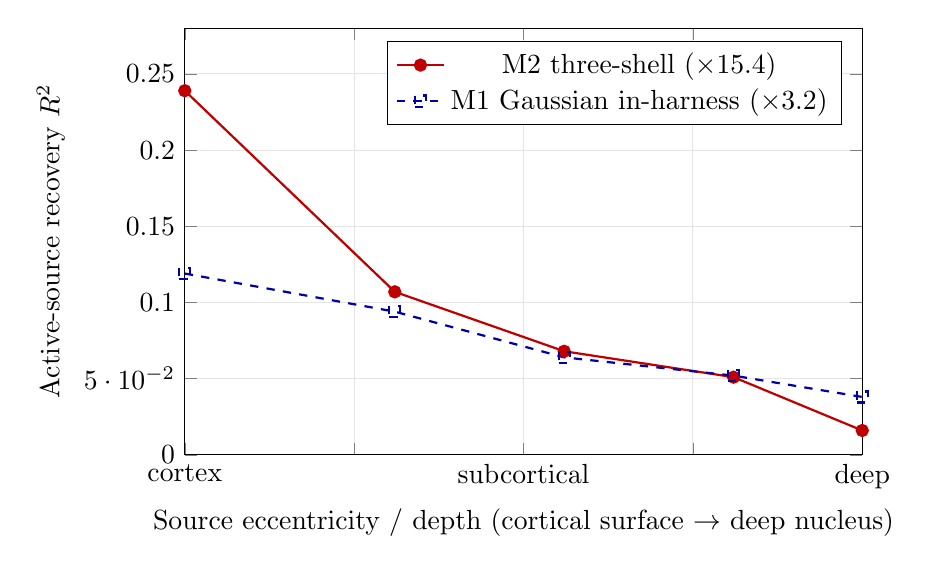
\begin{tikzpicture}
\begin{axis}[
  width=0.84\textwidth, height=7cm,
  xlabel={Source eccentricity / depth (cortical surface $\rightarrow$ deep nucleus)},
  ylabel={Active-source recovery $\Rsq$},
  xmin=0, xmax=1, ymin=0, ymax=0.28,
  xtick={0,0.25,0.5,0.75,1},
  xticklabels={cortex,,subcortical,,deep},
  legend pos=north east,
  grid=both, grid style={gray!20},
]
% Three-shell: ecc 0.95..0.10 -> R2 0.239,0.107,0.068,0.051,0.016 (x15.4)
\addplot[thick,red!75!black,mark=*] coordinates {
  (0,0.239) (0.31,0.107) (0.56,0.068) (0.81,0.051) (1,0.016)
};
\addlegendentry{M2 three-shell ($\times 15.4$)}
% Gaussian in-harness: 0.119,0.094,0.064,0.052,0.038 (x3.2)
\addplot[thick,blue!65!black,dashed,mark=square] coordinates {
  (0,0.119) (0.31,0.094) (0.56,0.064) (0.81,0.052) (1,0.038)
};
\addlegendentry{M1 Gaussian in-harness ($\times 3.2$)}
\end{axis}
\end{tikzpicture}
\caption{The depth wall. Active-source recovery $\Rsq$ vs.\ source eccentricity under
the naive Gaussian forward model (blue, dashed) and the physically grounded
three-shell model (red, solid), plotted from the measured 5-point ecc sweep
(Table~\ref{tab:depthwall}). The physically faithful model starts higher at the
surface but collapses \emph{faster} ($\times 15.4$ vs.\ $\times 3.2$), reaching
$\Rsq=0.016$ (chance) at the deep nucleus. Every plotted point is a measured ledger
value. The separately published Gaussian full-stack best-envelope collapses
$\times 8.4$ ($0.820\to0.098$); the three-shell wall exceeds even that.}
\label{fig:wall}
\end{figure}

\begin{figure}[h]
\centering
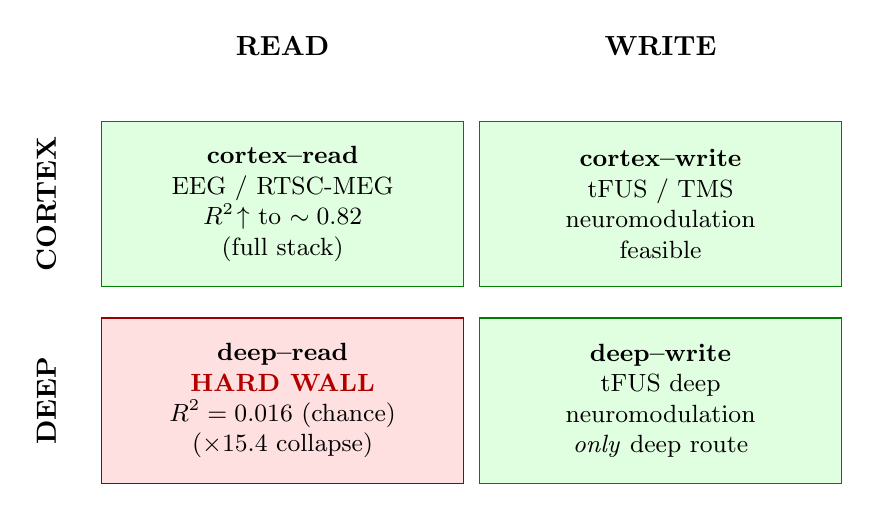
\begin{tikzpicture}[
  cell/.style={rectangle, draw, minimum width=4.6cm, minimum height=2.1cm,
               align=center, font=\small},
  ok/.style={cell, fill=green!12, draw=green!50!black},
  wall/.style={cell, fill=red!12, draw=red!60!black},
]
\node[font=\bfseries] at (2.3,2.0) {READ};
\node[font=\bfseries] at (7.1,2.0) {WRITE};
\node[font=\bfseries,rotate=90] at (-0.7,0) {CORTEX};
\node[font=\bfseries,rotate=90] at (-0.7,-2.5) {DEEP};

\node[ok]   (cr) at (2.3,0)    {\textbf{cortex--read}\\ EEG / RTSC-MEG\\ $\Rsq\!\uparrow$ to $\sim0.82$\\ (full stack)};
\node[ok]   (cw) at (7.1,0)    {\textbf{cortex--write}\\ tFUS / TMS\\ neuromodulation\\ feasible};
\node[wall] (dr) at (2.3,-2.5) {\textbf{deep--read}\\ \redbox{HARD WALL}\\ $\Rsq=0.016$ (chance)\\ ($\times15.4$ collapse)};
\node[ok]   (dw) at (7.1,-2.5) {\textbf{deep--write}\\ tFUS deep\\ neuromodulation\\ \emph{only} deep route};
\end{tikzpicture}
\caption{Read/write $\times$ depth capability matrix on the toy head. Three cells are
populated; the deep-read cell is the single hard-walled cell ($\Rsq=0.016$, chance).
The only non-invasive channel reaching deep structures is a \emph{write} channel
(tFUS deep neuromodulation; electric deep write requires invasive DBS). Source:
\texttt{AURA/AURA-AXES-INDEX.md} (17-app matrix), C15/C16 ledgers.}
\label{fig:matrix}
\end{figure}

%==========================================================================
\section{Finding}
\label{sec:finding}

\subsection{Primary: closed-negative on non-invasive deep control}
The pre-registered falsifier $F$ is \redbox{not satisfied}; the optimistic
hypothesis $H$ is \redbox{FALSIFIED (closed-negative)}. Neither escape clause holds:
\begin{itemize}[leftmargin=2em]
  \item \textbf{F1 fails:} the cortex/deep recovery ratio is $\times 15.4$ under the
        physically faithful three-shell model --- far above the $\lesssim 2\times$
        survival threshold --- and it \emph{steepened} relative to the in-harness
        Gaussian model ($\times 3.2$) and even the strongest Gaussian best-envelope
        ($\times 8.4$). The single direction that could have rescued $H$ (the ratio
        shrinking under a better model) is the opposite of what was measured. The
        explicit AURA-HEADMODEL conjecture that the toy ``over-states'' the wall was
        falsified by sign reversal.
  \item \textbf{F2 fails:} no non-invasive read modality reaches deep structures;
        deep recovery is at chance ($\Rsq = 0.016$). The only deep-reaching
        non-invasive channel is \emph{write}, not read.
\end{itemize}
The depth wall is therefore a \emph{real physical boundary}, attributable to the
resistive skull's spatial low-pass smearing (the $g_n \propto b^{2n}$ decay of the
radial-dipole scalp trace), not to a weak solver (the oracle solver shares the
collapse; $L1$/ISTA is strictly worse than ridge) nor to sparse sampling (the
saturation that would suggest a sampling ceiling is itself a Gaussian-model artifact
that vanishes under the three-shell model). Non-invasive whole-brain (deep) control
via electrode relocation or external fields is ruled out as a read pathway.

\subsection{Independent convergence with B7}
This depth-wall closed-negative independently converges with the AURA
\texttt{B7-intracortical-ceiling} finding, which reaches the same boundary from the
hardware side (an intracortical access ceiling: deep structures are an essentially
invasive target). Two methodologically distinct probes --- a forward/inverse
in-silico recovery sweep here, and the B7 ceiling analysis --- land on the same wall,
strengthening the ruling beyond a single model's idiosyncrasy.

\subsection{Positive complement 1: cortical-surface capability window}
On the cortical \emph{surface}, the gap to invasive grade is largely closable
non-invasively: heterogeneous-modality fusion (EEG-64 $0.329 \rightarrow$
RTSC-MEG-256 $0.764$), the dynamic-time joint-support lever ($+0.184$ at the cortical
layer), and channel-density scaling (non-saturating under faithful physics,
$0.19 \rightarrow 0.40$ out to 1024 contacts) combine to a near-invasive composite
$\sim 0.82$--$0.90$ on the toy head. This defines a \greenbox{cortical-surface
application window} (the C16 capability map): the regime where non-invasive
engineering is worth pursuing, and where 15 of 17 catalogued AURA apps already live.

\subsection{Positive complement 2: the write-only deep route}
The single non-invasive channel that touches the deep brain is transcranial focused
ultrasound as a \emph{write} (neuromodulation) channel, with the best deep residual
recovery ($\Rsq \approx 0.15$--$0.20$, vs.\ chance for every read modality). The
read/write asymmetry is the actionable design consequence: any non-invasive ``deep''
ambition must be a \emph{write} ambition (stimulation / modulation), because deep
\emph{reading} is hard-walled. Clinically, this is exactly the pattern in the AURA
app matrix --- cortical disorders (epilepsy, paralysis, blindness) are non-invasively
addressable, while deep-nucleus disorders (depression via raphe, Parkinson via STN)
remain invasive-DBS or tFUS-write only.

%==========================================================================
\section{Threats to Validity}
\label{sec:threats}

\paragraph{Toy head (spherical, Gaussian sources).} All numbers are $\Rsq$ on a
concentric-sphere head with synthetic Gaussian-distributed sources. A real head has
skull anisotropy, gyral folding, and CSF shunting that the sphere model omits. We
mark this explicitly: \textbf{real-head modelling is NOT-MEASURED.} However, the
qualitative direction is robust for a specific reason: the dominant physics of the
depth wall is the resistive skull's spatial low-pass, which the three-shell model
\emph{already} includes, and making the model more faithful (Gaussian
$\rightarrow$ three-shell) made the wall \emph{stronger}. Realistic boundary-element
models in the literature only add further smearing, never less. The
eccentricity-to-physical-depth (cm) mapping is a toy proxy, not calibrated to real
VTA/LC/raphe coordinates.

\paragraph{Synthetic, not recorded, data.} No real EEG/MEG/tFUS recordings were used.
\textbf{Real-data confirmation is NOT-MEASURED.} Only radial dipoles are modelled;
real cortex carries tangential components too, and skull-conductivity anisotropy
($\sigma_{\text{radial}}\ne\sigma_{\text{tangential}}$) is omitted.

\paragraph{No built-in $\Phi$ confirmation.} Recovery is scored by $\Rsq$, a
source-recovery proxy, not by a hardware- or hexa-builtin-verified integrated
information $\Phi$. \textbf{$\Phi$-builtin confirmation is NOT-MEASURED.} The claim
is about source recoverability, which bounds any downstream consciousness-proxy
read: you cannot read a deep $\Phi$ contribution you cannot recover the deep source
of.

\paragraph{Absolute vs.\ relative numbers.} The toy-scale absolute $\Rsq$ values
should be read as relative capability indices, not production-grade recovery
guarantees. The load-bearing results are the \emph{ratios and orderings} (deep
$\ll$ cortex; three-shell steeper than Gaussian; saturation absent under three-shell;
fusion $>$ baseline; write reaches deep, read does not), which are sign-stable across
both head models.

%==========================================================================
\section{Related AURA Axes}
\label{sec:related}

This paper sits on the AURA C-axis (non-invasive $\rightarrow$ invasive-grade). It
cites and integrates: C6 (multimodal breakthrough), C7 (prior-stack levers), C10
(gap-closure / saturation artifact), C13 (channel-density scaling), C15 (depth-wall
terminal), C16 (cortical capability map), C17 (deep-nuclei capability map), and B7
(intracortical ceiling, the independent convergence). It is orthogonal to the
A-axis electrode-position $\Phi$-proxy paper, which addresses scalp position rather
than depth and direction.

%==========================================================================
\section{Conclusion}
\label{sec:conclusion}

Within an in-silico toy-head testbed, the non-invasive depth wall is real and, if
anything, \emph{understated} by naive models. The optimistic hypothesis --- that a
relocated or chip-free non-invasive interface could reach invasive-grade deep access
--- is falsified as a \emph{read} pathway: deep recovery sits at chance
($\Rsq = 0.016$) and the collapse steepens ($\times 15.4$) under faithful physics,
while the apparent escape hatch (electrode saturation) is exposed as a modelling
artifact. The negative result is the finding, and it converges independently with
B7. The complementary positives sharpen, rather than soften, the ruling: the
cortical \emph{surface} is a near-invasive non-invasive capability window
($\sim 0.82$--$0.90$ composite), and the \emph{only} non-invasive route into the deep
brain is a \emph{write} channel (tFUS), defining a read/write depth asymmetry that
should steer all future AURA non-invasive-depth effort toward modulation, not
readout.

\bigskip
\noindent\textbf{Reproducibility.} All measured values are quoted verbatim from
AURA origin/main verdict ledgers (Section~\ref{sec:method}, ``Provenance''). The
forward/inverse harness is the AURA-DEPTH / AURA-HEADMODEL toy code
(\texttt{AURA/AURA-DEPTH/app/}, \texttt{AURA/AURA-HEADMODEL/app/}); numpy CPU,
8 seeds, SNR 20\,dB, \$0.

\bibliographystyle{plain}
\bibliography{refs}

\end{document}
